\section{Potenziometro circolare}
Il funzionamento è identico a quello di posizione lineare cambia il
fatto che ora si misura un angolo e non una distanza quindi la
relazione ora è la seguente:

	\[V=E\frac{\theta}{360\textdegree}\]

\subsection{Vantaggi}
L'unico vantaggio è la linearità fra la tensione fornita e l'angolo
misurato.
\subsection{Svantaggi}
Gli svantaggi sono, invece, l'ambiguità fra l'inizio e la fine (il
cursore passa da 360 a 0 gradi) e l'esistenza di una zona morta nella
quale non si può misurare per via dell'assenza di contatti.

% \section{Synchro} % FIXME tosto
\section{Encoder binario ed a codice di Gray}
Tramite un encoder è possibile misurare numericamente l'angolo
rilevato, per farlo si utilizza un disco così costituito: tanti
settori quanti sono gli angoli misurabili e tante corone quanti sono i
bit necessari per determinare tutti gli angoli misurabili. Dopo la
divisione alcune aree vengono oscurate per identificare gli zero della
codifica binario o gray. Il codice gray viene utilizzato quando si
vuole eliminare l'ambiguità fra una codifica e l'altra.

\begin{figure}[htbp]
	\centering
	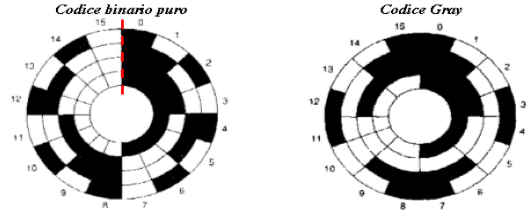
\includegraphics[scale=0.5]
			{img/encoder.png}
	\caption{Encoder binari ed a codice di
Gray\label{fig:encored}}
\end{figure}

Per la rilevazione della codifica vengono usate tante coppie di LED e
foto-transistor quante sono le corone utilizzate; dopo di che, vengono
opportunamente allineati di modo che ogni coppia faccia riferimento
solo ad una corona. Al movimento della corona grazie alle parti scure
è possibile rilevare la codifica dell'angolo.

\section{Encoder incrementale}
Questo tipo di encoder si differenzia dal precedente per l'utilizzo
di solo due corone concentriche suddivise in settori sfasati di un
quarto di periodo.

\begin{figure}[htbp]
	\centering
	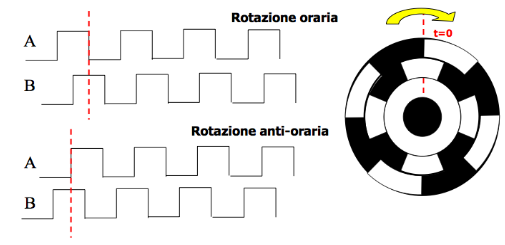
\includegraphics[scale=0.5]
			{img/encoderincr.png}
	\caption{Encoder incrementale\label{fig:encored}}
\end{figure}

In questo modo è possibile riconoscere gli incrementi e i decrementi
di angolo e quindi calcolare l'angolo finale. Indichiamo con $P$ il
fronte positivo e con $N$ il fronte negativo del segnale e con $S_1$
la corona esterna e con $S_2$ la corona interna; ne risulta la
seguente tabella di incrementi:

\begin{center}
\begin{tabular}{lll}
$S_1$ & $S_2$ & incremento\\
P & 0 & +1\\
P & 1 & -1\\
N & 0 & -1\\
N & 1 & +1\\
0 & P & -1\\
1 & P & +1\\
0 & N & +1\\
1 & N & -1
\end{tabular}
\end{center}

A partire dalla posizione di riposo, sarà facile calcolare l'angolo
ottenuto nelle rotazioni.
